\documentclass{report}

\usepackage[utf8]{inputenc} % allow utf-8 input
\usepackage[T1]{fontenc}    % use 8-bit T1 fonts
\usepackage{hyperref}       % hyperlinks
\usepackage{url}            % simple URL typesetting
\usepackage{booktabs}       % professional-quality tables
\usepackage{amsfonts}       % blackboard math symbols
\usepackage{nicefrac}       % compact symbols for 1/2, etc.
\usepackage{microtype}      % microtypography
\usepackage{xcolor}
\usepackage{amsmath}         % colors
\usepackage{listings}
\usepackage{graphicx}
\usepackage{multirow}
\usepackage{tabularx}
\usepackage{cleveref}
\usepackage{float}

\definecolor{codegreen}{rgb}{0,0.6,0}
\definecolor{codegray}{rgb}{0.5,0.5,0.5}
\definecolor{codepurple}{rgb}{0.58,0,0.82}
\definecolor{backcolour}{rgb}{0.95,0.95,0.92}

\lstdefinestyle{mystyle}{
    backgroundcolor=\color{backcolour},
    commentstyle=\color{codegreen},
    keywordstyle=\color{magenta},
    numberstyle=\tiny\color{codegray},
    stringstyle=\color{codepurple},
    basicstyle=\ttfamily\footnotesize,
    breakatwhitespace=false,
    breaklines=true,
    captionpos=b,
    keepspaces=true,
    numbers=left,
    numbersep=5pt,
    showspaces=false,
    showstringspaces=false,
    showtabs=false,
    tabsize=2
}

\lstset{style=mystyle}


\title{Distributed Databases Project}

\author{
    Jop Zitman\\
    Department of Computer Science\\
    Tsinghua University\\
    Beijing, China \\
    \and
    Borislav Pavlov\\
    Department of Computer Science\\
    Tsinghua University\\
    Beijing, China \\
}


\begin{document}

    \maketitle

    \begin{abstract}
        This report presents a distributed database system adept at handling both structured and unstructured data with high efficiency. At its core, the system integrates advanced technologies such as Kubernetes, MinIO, MongoDB, Redis, and FastAPI. It is architected to achieve scalability, high availability, and incorporates robust monitoring strategies. The design leverages Kubernetes orchestration, diversified databases, storage solutions, and a Python-based API. This results in a system that is not only performant and reliable but also capable of handling extensive data volumes and high concurrency. The system excels in managing various data types, boosted by efficient caching mechanisms for real-time responsiveness. Further, the integration of monitoring tools offers instantaneous insights, facilitating swift identification and resolution of issues. Performance evaluations affirm the system's competency in meeting the needs for effective large-scale data storing and serving.
    \end{abstract}

    \tableofcontents
    \pagebreak

    \section{Introduction and Motivation}
    The advent of distributed systems has revolutionized the way data is stored, accessed, and processed. As the digital universe expands exponentially, there is an incessant demand for systems that can handle vast and varied data types efficiently. This project seeks to address these needs by developing a distributed database system tailored to manage an extensive array of articles and user interactions. The envisioned system is not only required to handle high volumes of both structured and unstructured data but also ensure that data retrieval is both swift and reliable, accommodating a significant number of concurrent users. Furthermore, the system's architecture should be robust enough to maintain functionality even in the face of certain system failures, thereby ensuring a degree of fault tolerance crucial for maintaining service continuity.

    Achieving this ambitious set of objectives necessitates a multifaceted approach involving the development of a scalable API server for data access, the integration of structured and unstructured data stores, the implementation of effective caching mechanisms to expedite data retrieval, and a comprehensive solution for monitoring system components to guarantee optimal performance and reliability.

    This project is not just an academic exercise; it is a vital step towards understanding and leveraging cutting-edge big data management techniques, with profound implications for real-world applications. By dissecting and reconstructing the complexities of distributed databases, we aim to contribute meaningfully to the field's body of knowledge and pave the way for innovative solutions to data management challenges.


    \section{Problem Statement}
    Central in our investigation is the generated dataset for a news site. The generated data includes a number of \textbf{articles} with their text, image, and/or video content. In addition, the \textbf{user} accounts and the articles which they \textbf{read} are provided. Besided the generated data, requirements also include the need of generating article metrics and popularity rankings. Summarized, this gives us the following tables:

    \begin{itemize}
        \item \textbf{User}: Capturing personal information about users, like their name, gender, email, phone, etc.
        \item \textbf{Article}: Stores details about the articles, like their title and tags with links to images and videos.
        \item \textbf{Read}: A relational table capturing article reads for every user including some meta information about how long the user took to read it and whether the user liked it.
        \item \textbf{Be-Read}: As an aggregate of the \textbf{Read} table, it reflects comprehensive reader metrics, including read counts, agreements, and shares. This data is vital for understanding content popularity and user interaction trends.
        \item \textbf{Popular-Rank}: Aggregating \textbf{Be-Read}, this table synthesizes interaction data to rank content according to various metrics, providing insights into what is trending each day, week or month.
    \end{itemize}

    With the following entity relationship diagram in \Cref{fig:reference-entity-relation-diagram}.

    \begin{figure}[H]
        \centering
        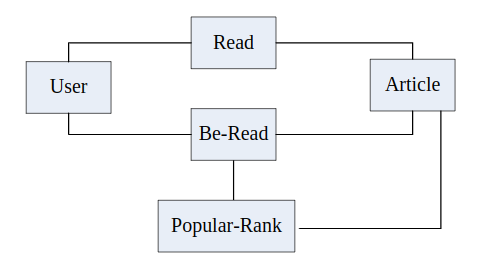
\includegraphics[width=0.5\textwidth]{images/reference-entity-relation-diagram}
        \caption{Reference Entity Relation Diagram}
        \label{fig:reference-entity-relation-diagram}
    \end{figure}

    And each of the tables should be sharded by:

    \begin{itemize}
        \item \textbf{User}: Horizontally fragmented by region.
        \item \textbf{Article}: Horizontally fragmented by region.
        \item \textbf{Read}: Fragmented based on and with the same allocation schema as User table. Without replication.
        \item \textbf{Be-Read}: Horizontally fragmented by category, with science articles being in both shards.
        \item \textbf{Popular-Rank}: Fragmented based on granularity.
    \end{itemize}

    Considering the loosely described reference infrastructure architecture provided in \Cref{fig:reference-infrastructure-architecture}, we see that we need the following stack:

    \begin{itemize}
        \item Unstructured Data Management Layer (Hadoop HDFS)
        \item Structured Data Management Layer (DBMS)
        \item Caching Layer (Cache)
        \item Application Layer (APP)
        \item Some system to orchestrate these layers
    \end{itemize}

    \begin{figure}[H]
        \centering
        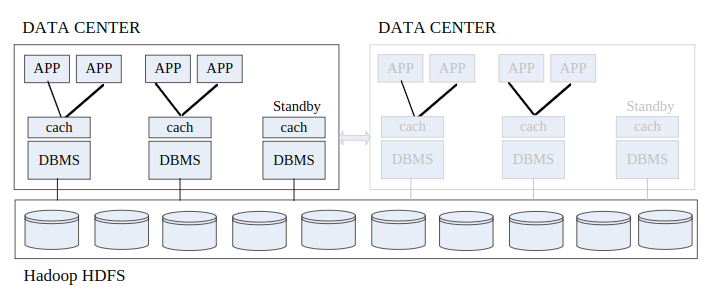
\includegraphics[width=\textwidth]{images/reference-architecture}
        \caption{Reference Infrastructure Architecture}
        \label{fig:reference-infrastructure-architecture}
    \end{figure}

    The unstructured data is large files such as videos, images, and article text. The system should support large volume data transfers for these files.

    For the functional requirements, we need to support bulk data loading, data insert/update/query, and monitoring of the servers and data.

    Optional (advanced) requirements (see \Cref{sec:advanced-requirements}) include Hot/Cold Standby DBMSs for fault tolerance, upscaling/downscaling DBMSs, and cross DBMSs data migration.

    \section{Proposed Methodology}
    To construct such system that meets these requirements, we propose an integrated solution comprising several cutting-edge technologies, each selected for its proven efficacy and relevance to the project's objectives. We will first discuss the rationale behind each technology choices and then elaborate on how these technologies will be integrated to create our system.

    \subsection{Technology Choices}\label{subsec:technology-choices}
    This paragraph introduces the choices of technologies that we made and comparisons of our choices to other existing solutions (i.e. literature review).

    \subsubsection{Containerization with Docker}
    Docker has become a go-to solution for portable applications. By leveraging existing computing concepts around containers, particularly in the Linux world, using primitives known as cgroups and namespaces, Docker reduces the overhead of creating and maintaining full virtual machines for running applications. This standardization of containerization has made the complex concepts of containerization more accessible and efficient for contemporary development needs. For instance, Docker's containerization technology is foundational to ensuring that our application is portable, consistent, and isolated from environmental inconsistencies across development and production platforms. This modularity is critical for testing, deployment, and allowing each component in a distributed system to be developed and deployed independently. In addition, the adaptability of the Docker Engine, supports responsive development and scaling, as Docker containers can be executed in diverse environments, from a developer's local laptop to various cloud providers. Finally, the modularity of Docker containers simplifies the process of scaling containers due to the ease and speed of creating new Docker containers.

    An alternative would be to use a Virtual Machine (VM) based deployment with a VM builder like Packer or Ansible to create portable and consistent VM images. The downside with such solution would be that these VMs are relatively large compared to Docker containers and that their boot time is larger than Docker too (slow scalability). It might also be a waste to horizontally scale entire VM's, since we don't actually want to scale the OS layer.

    We could also consider a solution like Amazon Lambda functions to deploy isolated parts of code, but this may be difficult to integrate with other parts of the project.

    Concluding, Docker's emergence has significantly accelerated the adoption of containerization technology. By abstracting complex containerization concepts into a user-friendly format, it has become an industry standard for containers, offering simple developer tools and a universal packaging approach. The widespread adoption of Docker underscores its importance as a tool for modern software development, testing, deployment, and scaling.

    \subsubsection{Orchestration with Kubernetes}
    Kubernetes stands at the forefront of container orchestration technologies, automating various manual processes related to managing containers such as scheduling, launching, scaling, and healing. It can be deployed on separate compute nodes, or simply taken as a service (e.g.\ Google Kubernetes Engine), providing a central API to manage Docker containers across all nodes. It is capable of handling multiple groups of containers across these nodes, providing essential features like networking, service discovery, load balancing, and storage orchestration. Every such feature is implemented as a primitive build block that rely on the Kubernetes API, where this API is commonly extended with custom so-called Kubernetes Operators that provide more control or features (e.g. Knative Serving and Eventing Framework).

    Other Orchestration platforms for Docker include Docker Compose, as it also includes many networking, volumes, etc. abstraction. We feel that it is not suitable for autoscaling out-of-the-box, while however this may be possible with third-party extensions. In addition, we like the challenge of using Kubernetes for this project such that we can learn more about it.

    In summary, Kubernetes' extensive ecosystem and its ability to streamline deployment, scaling, and operations of application containers render it an indispensable tool for automating and managing the lifecycle of containerized applications, ensuring the system's reliability and scalability.

    \subsubsection{Package Management with Helm Charts}
    Helm enhances Kubernetes's capabilities by facilitating the definition, installation, and upgrade of even the most complex Kubernetes applications. Helm simplifies the management of creation, packaging, configuration, and deployment of applications and services to Kubernetes clusters through Helm Charts. These charts are collections of Kubernetes YAML files designed to simplify the deployment process. It also tracks the versioned history of each chart installation and change, enabling comprehensible commands to roll back to a previous version or upgrade to a newer one, thus maintaining consistency and reliability in deployments.

    Helm Charts are created and maintained by a range of contributors including individual developers, organizations, cloud service providers, and technology vendors. Among these, Bitnami is a prominent contributor, offering a wide range of pre-packaged, production-ready Helm charts for various applications. These charts are known for their quality and reliability, ensuring that applications deployed using Bitnami's charts meet high standards of security and performance.

    The alternative is to use Kustomize, a completely logic-less alternative to Helm Charts. While it may be less complex than Helm Charts, there are not as many community-built Kustomize releases for the applications that we want to deploy.

    Overall, Helm significantly contributes to the Kubernetes ecosystem by offering a streamlined, efficient method for package management, ultimately enhancing the management of containerized applications. Its wide adoption underline the collaborative and community-driven approach in managing and deploying applications in containerized environments.

    \subsubsection{Unstructured Data Management with MinIO}
    MinIO offers an efficient and scalable solution for managing unstructured data with its high-performance, S3 compatible object storage system. It is Kubernetes-native, providing a consistent object storage interface across multiple cloud providers, on-premise, and at the edge. MinIO is recommended for complete S3 API functionality for object storage on Kubernetes. Its lightweight architecture allows it to run efficiently on low CPU and memory resources, enabling the hosting of a large number of tenants on shared hardware. This makes MinIO particularly effective in environments where resource efficiency and scalability are crucial. In addition, it provides full bucket or cluster replication, and has data fault-tolerance enabled by default using a bit-parity solution similar to RAID5/6. By supporting all core S3 features, it easy to integrate with existing S3 frameworks and easy to replace with any fully managed cloud provided object storage (considering its AGPL licence and relatively high commercial license cost).

    In comparison to existing solutions like Hadoop HDFS, we feel that S3 is a better fit for modern solutions. The Docker image for HDFS has not been updated in years and the deployment documentation is rather complex. Amazon DynamoDB could be another option for unstructured data, as it could also be used for structured data. Though we believe that these 2 data types are so different that the solution should be different too (separation of concerns). It is also more conventional to store images and videos in S3. We both have experience with S3 too.

    In summary, MinIO's high performance, robust fault tolerance mechanisms, and compatibility with a variety of cloud storage services make it a crucial component for managing unstructured data in containerized environments. Its integration with Kubernetes enhances its capability to provide reliable and scalable object storage solutions, addressing the complex and varied data management needs of contemporary systems.

    \subsubsection{Structured Data Handling with MongoDB}
    MongoDB's flexible, document-oriented structure makes it particularly adept at managing structured data in our system. It is a distributed database at its core level, which stores the data into JSON-like objects, meaning that it is also a NoSQL database. Its powerful indexing and querying capabilities, and support for complex aggregations and transactions ensure that our structured data is handled efficiently and effectively. The easy of sharding different tables across nodes makes it an easy choice for our requirements. The Bitnami Helm chart is a popular, well-documented option for deploying MongoDB, offering various configurations like standalone, replica set, or replica set with arbiters, simplifying the deployment and management of MongoDB within Kubernetes.

    The data generation was provided in MongoDB and Postgres format. Considering that Postgres does not support sharding, the choice was easy to make.

    \subsubsection{Caching with Redis}
    Redis, an in-memory key-value data store provides a performant solution for short-lived data, such as message queues or caches. By using an in-memory database for the most frequently queried data, we can accelerate data retrieval and reduce load on the databases. Its integration with Kubernetes ensures scalable and efficient management of cache instances, further optimizing the performance and responsiveness of applications. This makes it an ideal choice for caching needs.

    An popular alternative would be memcached, but memcached does not support replication, which may impact the efficiacy of its use as a cache in a high load environment.

    \subsubsection{API Development with FastAPI}
    We choose to use Python to develop the API because of the high number of third party packages available for the components that we use and because it allows for extremely high development speed.

    For the API, FastAPI is an excellent choice for bootstrapping projects due to ease of use. Its asynchronous handling is particularly beneficial for IO-bound tasks, common with interactions in MongoDB, Redis, and S3. The framework's straightforward design, complete with automatic API documentation, significantly eases the development and management of complex services. Moreover, it provides documentation by integration of Swagger UI and ReDoc automatically generated based on the type hints and function signatures, making it easy to understand and test the API. Thus, FastAPI stands out as a robust, efficient, and developer-friendly option for building APIs in demanding and dynamic environments.

    Note that FastAPI may not be a good choice for large scale enterprise applications, due to it being so simple. For large codebases, one may look at projects such as Django. Considering that the focus of this project should be on the database integration, we deemed the ease of development the most important factor in choosing an API framework.

    \subsubsection{Monitoring}
    In a distributed system project, monitoring plays a crucial role in ensuring the performance and reliability of services. Monitoring is the real-time collection of metrics and logs from a system, providing insights into its health and performance. It allows operators to identify and resolve issues before they have large impact on users. Centralized monitoring is particularly important in distributed systems, where the complexity of the system and the number of components make it difficult to identify and resolve issues without proper monitoring.

    \textbf{Metrics}:
    Prometheus is a key tool in this domain, serving as an open-source monitoring and alerting toolkit with a powerful time-series database and query language. For this project, we decided to use Prometheus as a metrics scraping platform due to its popularity, ease of use, and compatibility with Kubernetes and many other open-source applications (many projects provide prometheus metrics endpoints).

    \textbf{Logging}:
    Logging allows for the collection of events and messages from a system, providing a record of its activity, such as errors or informational messages. It is crucial for monitoring and troubleshooting, allowing operators to identify and resolve issues. Loki is an open-source, horizontally scalable, highly available log aggregation system inspired by Prometheus. It is designed to be cost-effective and easy to operate, using labels to organize log streams and queries to filter log streams, making it highly efficient and scalable. Unfortunately, we no longer had time to properly test and debug the Loki deployment, so we have omitted it from this project.

    \textbf{Alerting}:
    Alerting is a crucial component of monitoring, allowing operators to be notified of issues and resolve them before they impact users. AlertManager is an open-source alerting system that works with Prometheus to send alerts to various receivers, including email, Slack, and more. It allows for the grouping and deduplication of alerts, ensuring that operators are not overwhelmed by a flood of alerts. AlertManager is highly configurable, allowing for the creation of complex alerting rules and routing trees, making it a powerful tool for monitoring and alerting.

    \textbf{Dashboarding}:
    The facto choice for dashboard management in the Prometheus ecosystem is Grafana, an open-source visualization platform that allows users to create, explore, and share dashboards that visualize the metrics data collected by Prometheus. Grafana is highly customizable, with a wide range of plugins and community-built dashboards, making it an ideal choice for monitoring and visualization. It also integrates with AlertManager, allowing for the creation of dashboards that display alerts and their status.

    \textbf{Prometheus Operator}
    These tools are deployed using the Prometheus Operator, a method that simplifies the deployment and management of Prometheus, Grafana, and Alertmanager in Kubernetes environments. The operator provides a cluster-wide framework for lifecycle management, including resource deployment and configuration, and offers a more automated and scalable approach to monitoring. Among others, this setup introduces the crucial Kubernetes ServiceMonitors and PodMonitors. They define how groups of services pr pods should be monitored by Prometheus, specifying the endpoints to scrape metrics from, along with the scraping interval and other parameters. They are particularly useful for monitoring services that dynamically scale within Kubernetes. Many Bitnami Helm charts provide ServiceMonitors and PodMonitors out of the box, making them an ideal choice for monitoring.

    Together, Prometheus, Grafana, and AlertManager, when deployed via the Prometheus Operator and utilizing ServiceMonitors and PodMonitors, create a powerful, scalable monitoring solution that can adapt to the changing landscape of a distributed system, providing vital metrics and alerts to maintain system health and performance.

    We choose this stack because we have experience with it and because many of the Bitnami charts support this stack out-of-the-box. We believe that the monitoring stack you choose will always be impacted by the other integration you use. For example, you may be more geared towards the ELK stack if you use other ElasticSearch products (such as its vector store). Some other stacks for reference:

    \begin{itemize}
        \item ELK (ElasticSearch, LogStash, Kibana)
        \item TIG (InfluxDB, Telegraf, and Grafana)
        \item Datadog
        \item and many more
    \end{itemize}

    \subsection{System Architecture}
    This section provides an overview of the deployment and interaction of various components within the system. Our architecture is designed for scalability, high availability, and robust monitoring, utilizing a combination of Kubernetes, databases, storage solutions, and a Python API.

    \subsubsection{Deployment Overview}
    The following components are deployed in our system:

    \textbf{Kubernetes on Minikube:} Minikube is used to deploy a Kubernetes cluster on a local machine. This will allow us to test and develop our system in a local environment before deploying it to a cloud provider.

    \textbf{Monitoring Tools:} Prometheus operator with default Grafana and AlertManager.

    \textbf{Minio S3 Storage:} Default MinIO provided chart configured with 4 nodes, each with 2 drives, and service-monitors for Prometheus.

    \textbf{MongoDB:} The infrastructure for supporting sharding in MongoDB requires several components, namely Mongos (MongoDB Router), Config Servers, and Shards. The Config Server Mongo instances keep track of all the metadata related to the shard instances, which register themselves with the config server as soon as they are spawned. The MongoDB Router acts as a middleware between the client and the data, communicating to the config server to know in what shard the data is placed when requested. We use the Bitnami Helm chart to deploy 3 routers, 3 config servers, 2 shards, each with 3 replicas.

    \textbf{Redis:} Deployed with 1 master and 3 replicas without persistence and with service and pod monitors included.

    \textbf{API:} The default Helm Chart has been used to deploy a Deployment, Horizontal Auto Pod Scaler to provide a scalable solution.

    \subsubsection{Component Interaction}

    Kubernetes orchestrates all components, managing their lifecycle, scaling, and networking. The Python API interacts with Minio for object storage, MongoDB for persistent data storage, and Redis for caching. Monitoring tools are integrated throughout, with Prometheus gathering metrics, Grafana for visualization, and Alertmanager handling alerts.

    \begin{figure}[H]
        \centering
        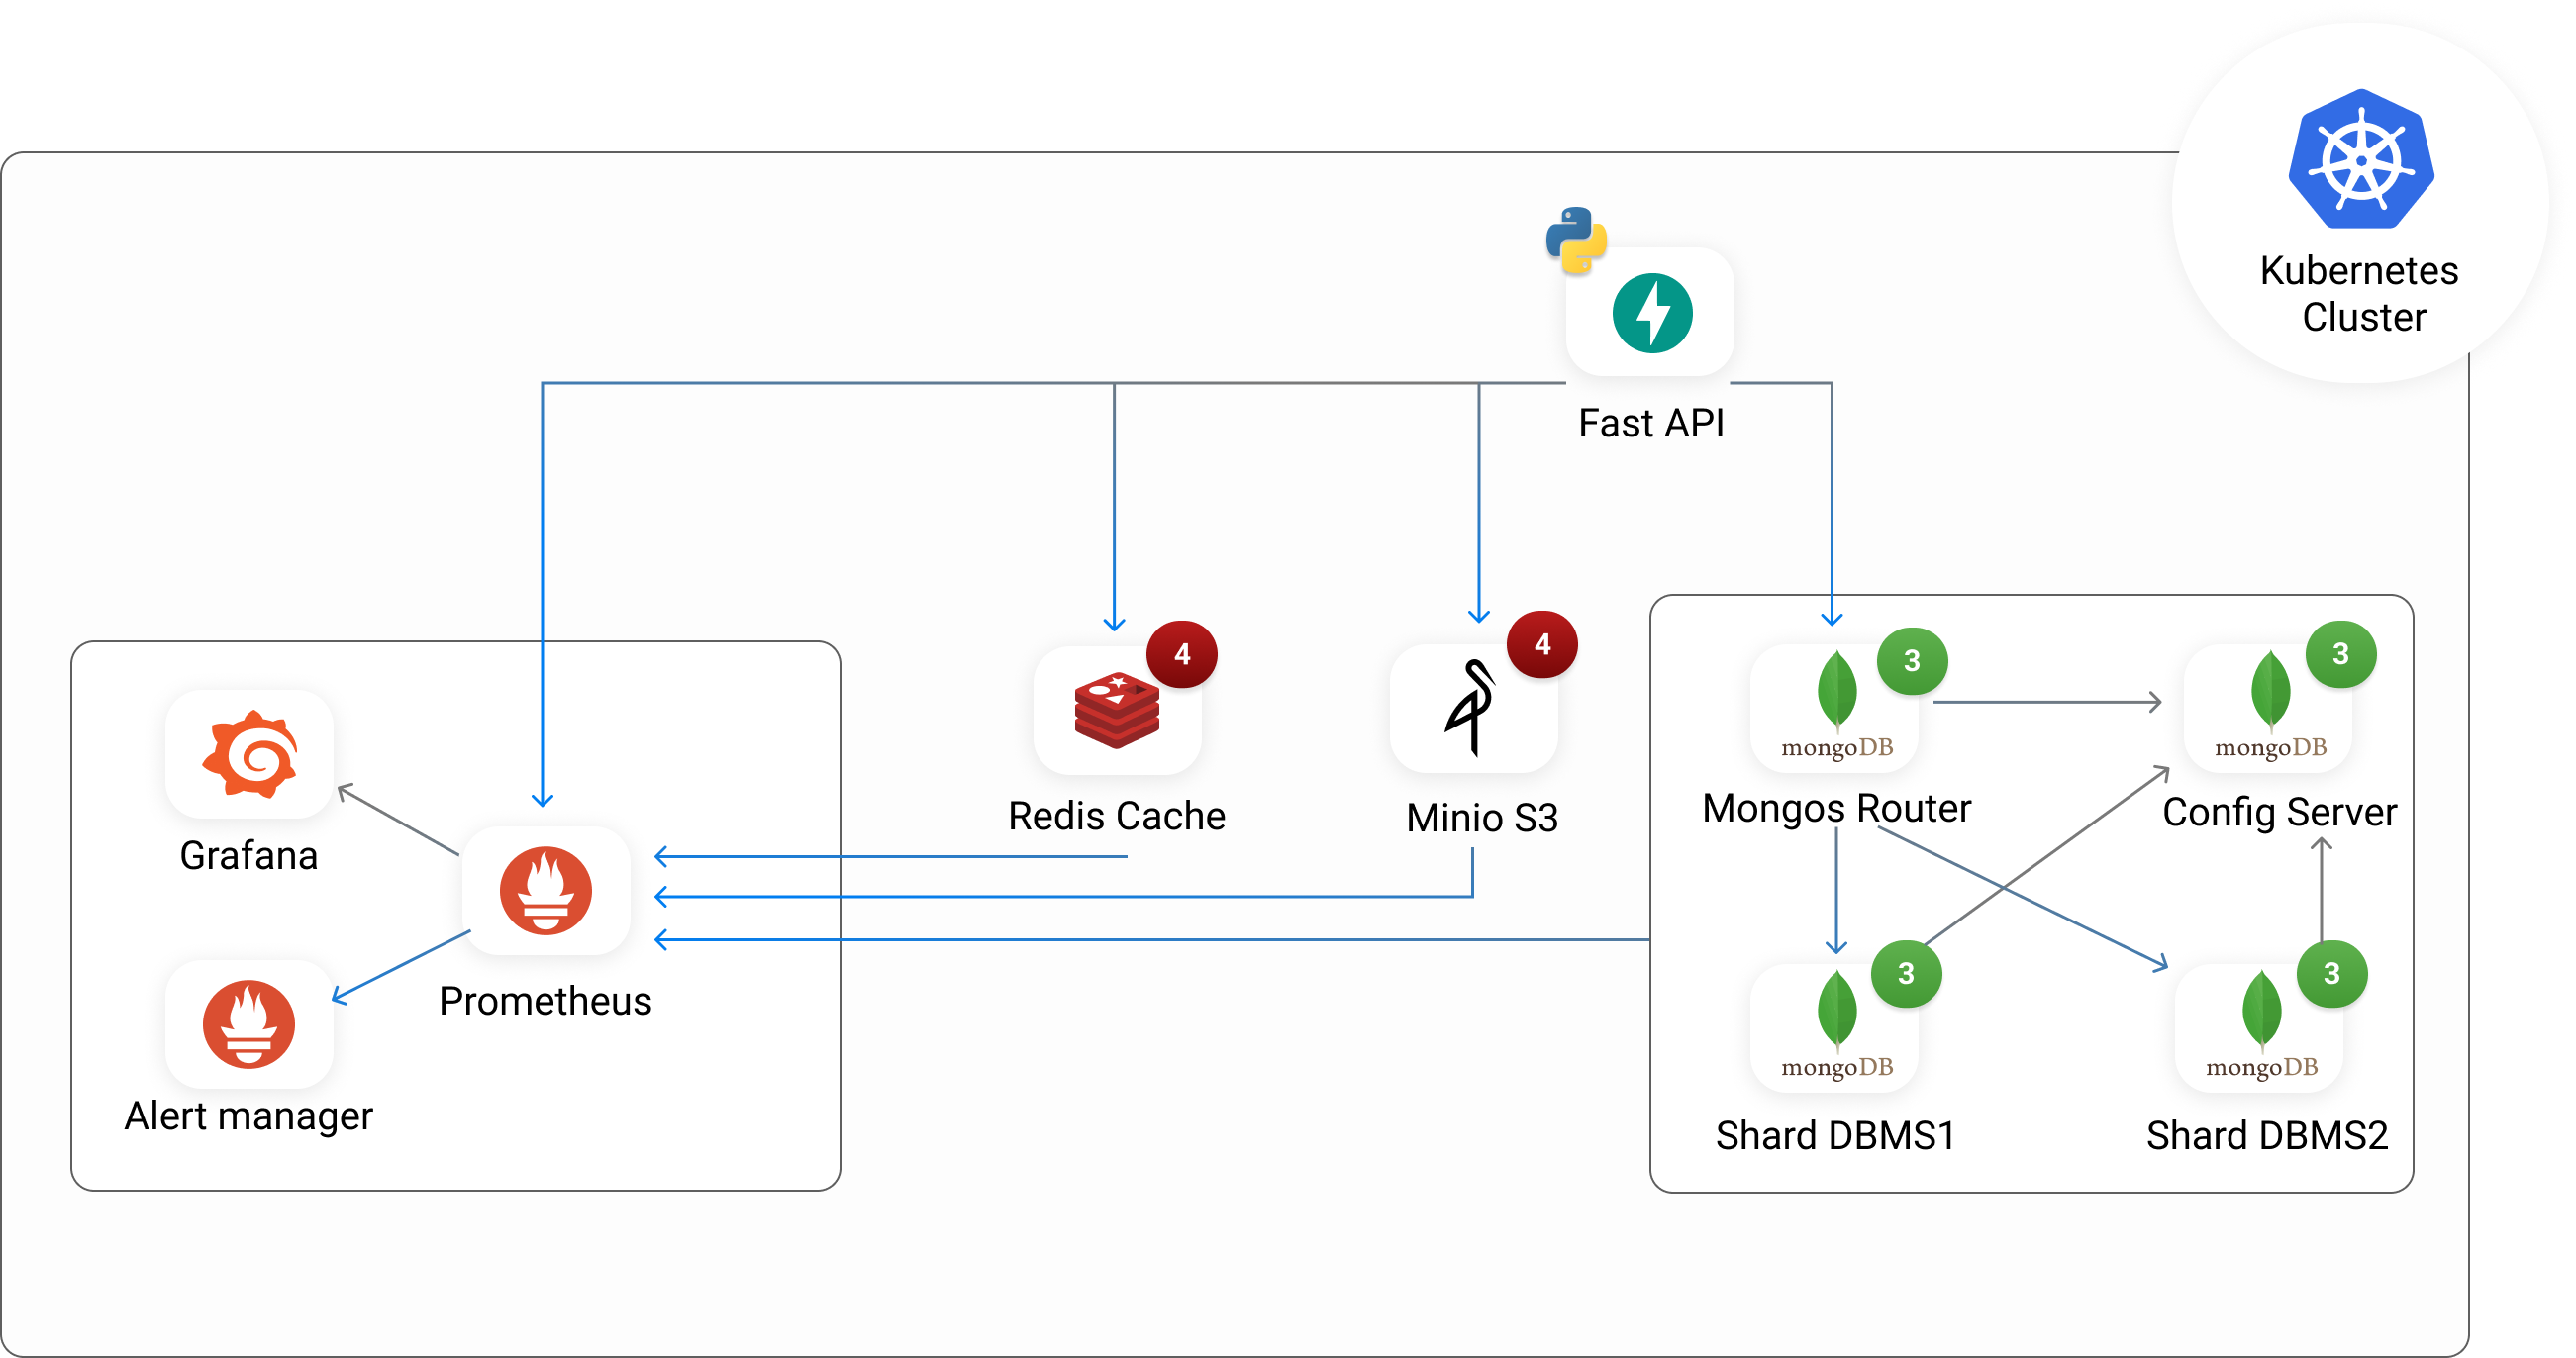
\includegraphics[width=\textwidth]{images/architecture}
        \caption{Solution Infrastructure}
        \label{fig:cluster}
    \end{figure}

    \subsection{Application Configuration}

    The entire source code has been attached to this report. The following sections describe implementation details for each of the requirements.

    \subsubsection{Unstructured Data Management / MinIO}
    All articles, videos, and texts should be stored in the unstructured data layer, for which we use MinIO. We deploy MinIO with the MinIO provided Helm Chart, for which our used Helm values can be found in the s3 folder. We initialize it with an empty bucket called media, without any versioning, object-locking, or any manual replication settings. A set of default credentials is used. For demonstrative purposes, we create several data nodes and attach multiple drives to each node.

    In a distributed MinIO setup, each server has a complete understanding of the distributed topology, allowing any node to handle requests and route internal communications to other nodes as necessary. There is no specific leader node or master; instead, the architecture is designed so that each node can equally participate in handling client requests and internal operations, reflecting a peer-to-peer approach.

    For the bulk data loading of the generated text, image, and video data, we've provided a script in the `s3-seed` directory to upload all to the created bucket.

    \subsubsection{Structured Data Management / MongoDB}
    \textbf{Aggregation pipelines}: essentially a powerful feature that allows processing and transformation of data within the database. Aggregation pipelines provide a framework for performing complex data manipulations, aggregations, and transformations on documents in a MongoDB collection. An aggregation pipeline is a series of stages through which documents pass, with each stage performing a specific operation on the data. These stages are executed sequentially, and the result of each stage becomes the input for the next stage. The pipeline stages can include operations such as filtering, sorting, grouping, and applying various transformations.

    To fulfill the requirements of the project, several MongoDB aggregation pipelines were utilized (\Cref{subsec:appendix-aggregation}). These results can be viewed once as a view, but also stored on disk as another table (on-demand materialized views), again allowing them to be sharded across different nodes. Whenever the original table is updated, we can rerun the aggregation pipeline to update the views. We can also run aggregation pipelines in API queries to join several tables together.

    All the different pipelines used are summarized below:
    \begin{enumerate}
        \item \textbf{Table Read/Article Alternation}: The requirement is to shard the Read and Article table by region, however, these tables don't include this property. Hence, a lookup is performed in the User table then the region field is projected and merged into the tables.
        \item \textbf{Table Be-Read Generation}: The Be-Read table is generated by querying the Read table, grouping all items by article ID, and counting the total number of reads, shares, comments, and agreements. Finally, the result is written into the Be-Read table, including the category field as it is needed to shard the table.
        \item \textbf{Table Popular-Rank Generation}: The Popular Rank table is generated by the following aggregation pipeline, starting from the Be-Read table and doing it for each granularity:
         \begin{enumerate}
            \item Compute the unique period identified for specific granularity - day, week, month
            \item Group by period, compute the total interactions by summing together the total reads, comments, shares, and agreements, and push each related user who read the article into a list
            \item Sort the items by the number of total interactions with the most one starting from the beginning
            \item Project the fields and merge them into the new table Popular Rank
        \end{enumerate}
        \item \textbf{Table Science Articles}: One of the requirements is to allocate science articles into every shard in the cluster, however, MongoDB doesn't support duplicated data as it is against the design principles behind the sharded cluster. Hence, a new on-demand materialized view is created by getting all the articles with the category science from the Article table and putting them into a new table Articles-Science. The same strategy is applied for the Be-Reads table as it has to be sharded in the same way as the Article table.
    \end{enumerate}

    \begin{table}[H]
        \centering
        \begin{tabularx}{\textwidth}{|c|c|X|}
            \hline
            \textbf{Table Name} & \textbf{Shard} & \textbf{Criteria} \\
            \hline
            User & Shard1 & Region = "Beijing" \\
            & Shard2 & Region = "Hong Kong" \\
            \hline
            Article & Shard1 & Category = "Science" \\
            & Shard2 & Category = "Science" and "Technology" \\
            \hline
            Read & Shard1 & Region = "Beijing" \\
            & Shard2 & Region = "Hong Kong" \\
            \hline
            Be-Read & Shard1 & Category = "Science" \\
            & Shard2 & Category = "Science" and "Technology" \\
            \hline
            Popular-Rank & Shard1 & Temporal Granularity = "day" \\
            & Shard2 & Temporal Granularity = "week | month" \\
            \hline
        \end{tabularx}
        \caption{Table Sharing Criteria}
        \label{tab:table-sharing}
    \end{table}

    The sharding configuration was implemented using the utility functions of Mongo shell. Scripts were created for consistent and automated deployment for both the aggregation pipelines and the sharding (\Cref{subsec:appendix-sharding}).

    \subsubsection{Python API}
    The following endpoints were created in the Python API:
    \begin{enumerate}
        \item Get Users: Querying User collection with or without filters
        \item Get Articles: Querying Article collection with or without filters, including getting text, images, and videos accordingly from the Minio S3 buckets
        \item Get Reads: Querying Read collection with or without filters, including joining of User and Article collection (including getting data from Minio S3 buckets)
        \item Get Be-Reads: Querying Be-Read collection with or without filters, including joining of Article table, including getting data from Minio S3 buckets
    \end{enumerate}

    \subsubsection{Redis}
    We use the existing Python package fastapi-cache (\url{https://github.com/long2ice/fastapi-cache}) that acts as a middleware for FastAPI that creates cache keys based on the request, checking in Redis before executing our API code. If the key did not exist, this package will automatically add our response to Redis.

    \subsubsection{Monitoring}
    For metric insights, there are many community-provided dashboards that work with our solution. In Grafana, it is easy to import these dashboards and visualize the metrics. \Cref{fig:dashboard-minio} shows a MinIO dashboard, \Cref{fig:dashboard-mongodb} shows a MongoDB dashboard, and \Cref{fig:dashboard-redis} shows a Redis dashboard. Kubernetes dashboards are included by default.
    \begin{figure}[H]
        \centering
        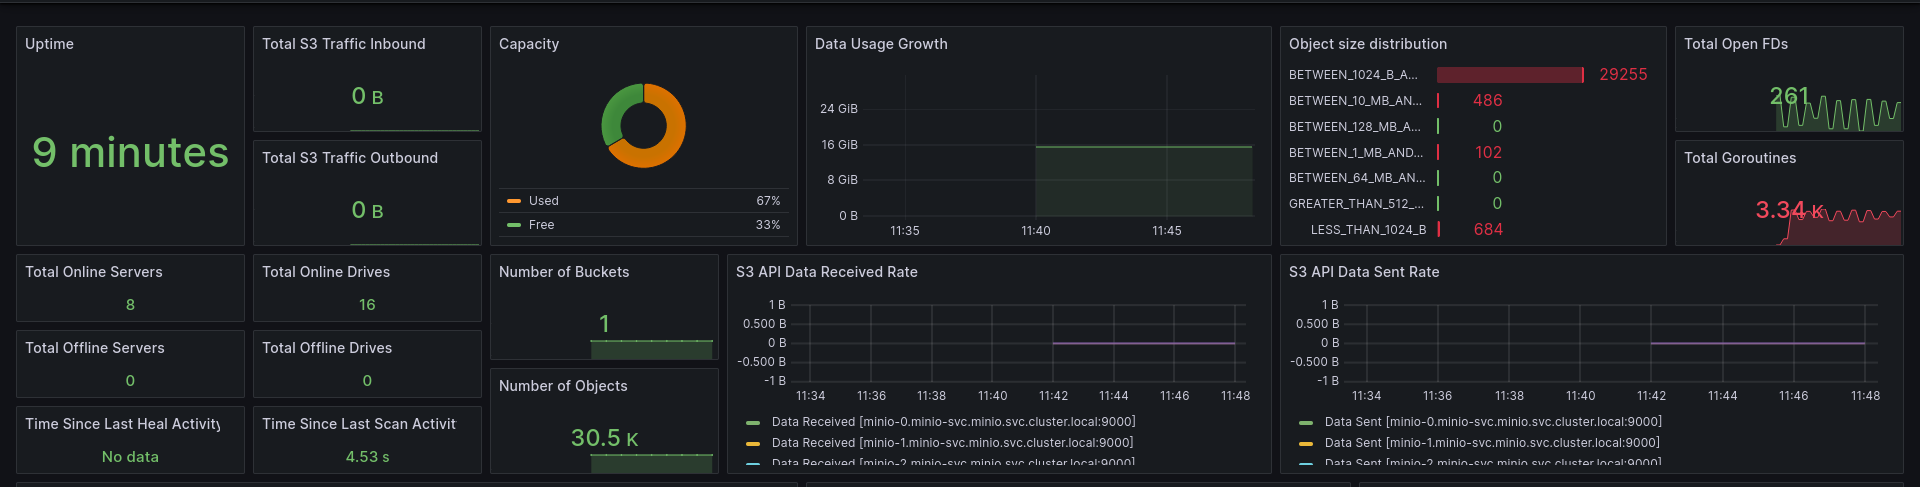
\includegraphics[width=\textwidth]{images/dashboard-minio}
        \caption{MinIO: \url{https://grafana.com/grafana/dashboards/13502/}}
        \label{fig:dashboard-minio}
    \end{figure}
    \begin{figure}[H]
        \centering
        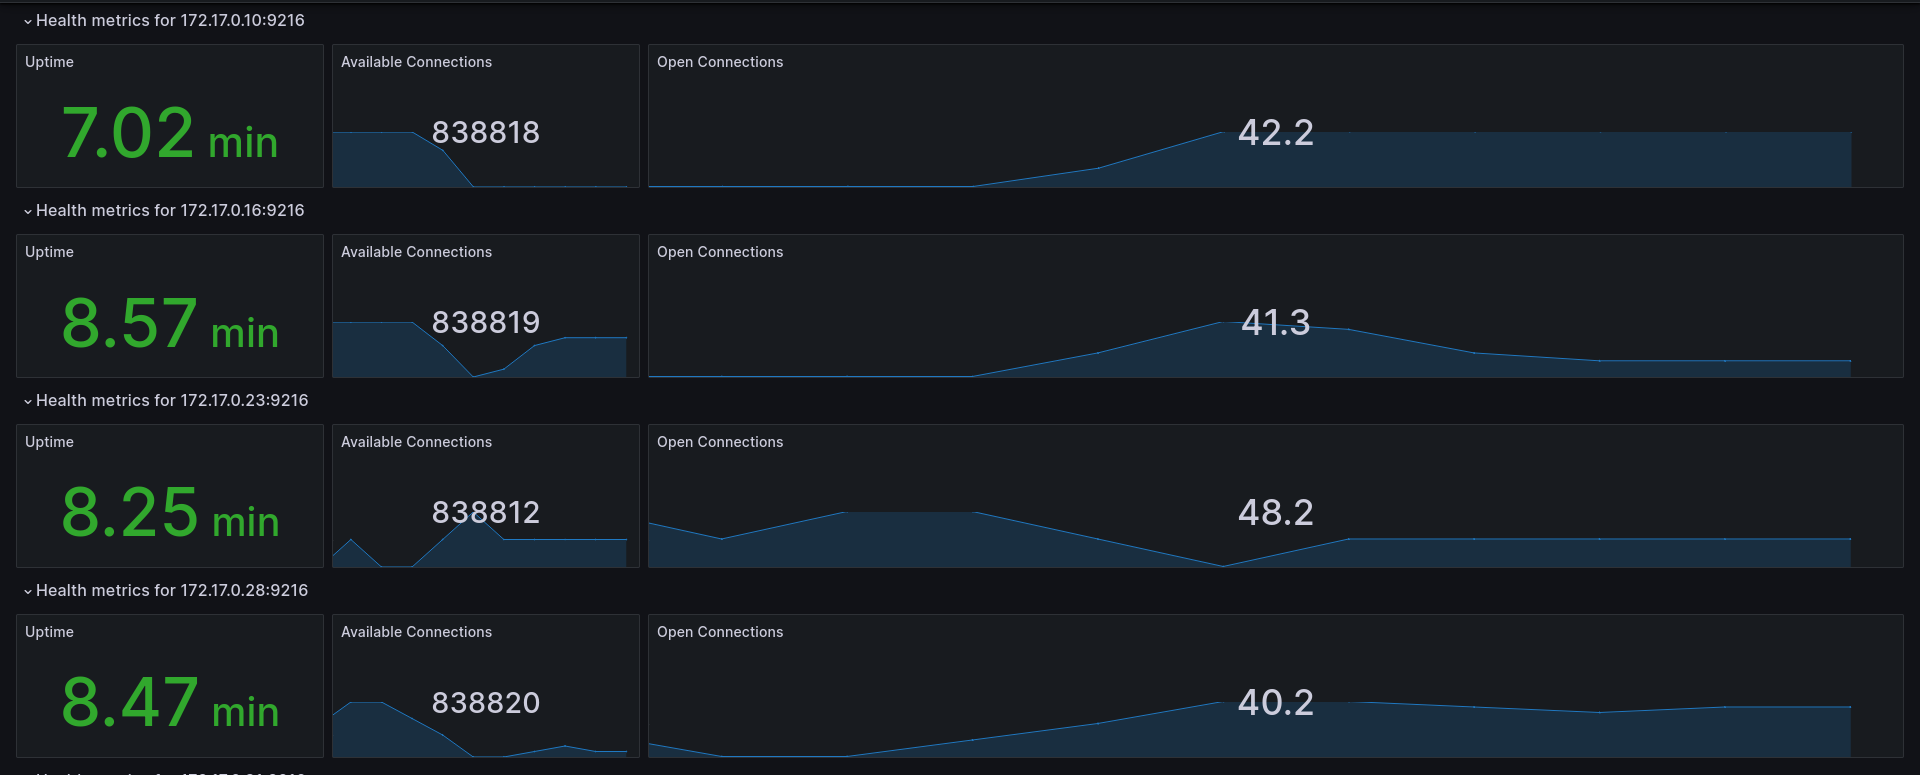
\includegraphics[width=\textwidth]{images/dashboard-mongodb}
        \caption{MongoDB: \url{https://grafana.com/grafana/dashboards/12079/} any "percona" dashboard works.}
        \label{fig:dashboard-mongodb}
    \end{figure}
    \begin{figure}[H]
        \centering
        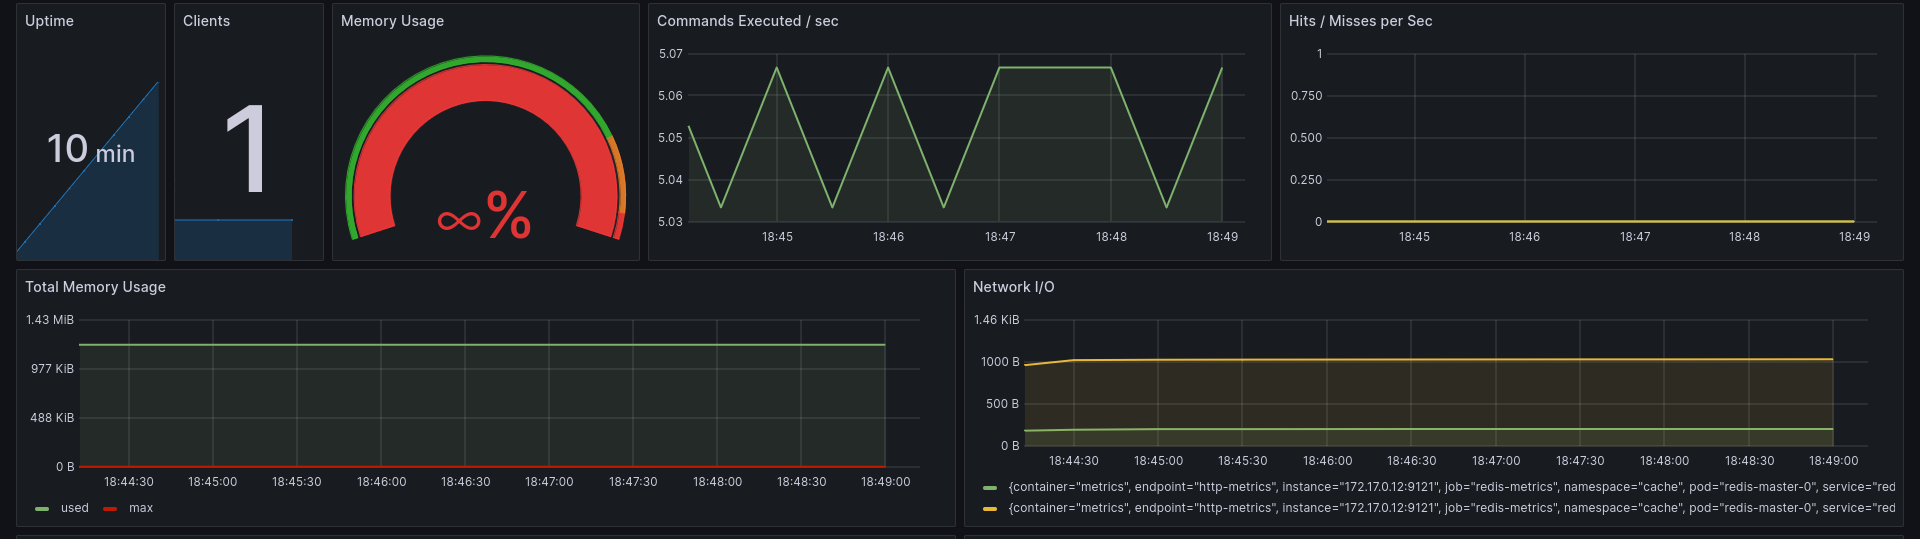
\includegraphics[width=\textwidth]{images/dashboard-redis}
        \caption{Redis: \url{https://grafana.com/grafana/dashboards/11835/}}
        \label{fig:dashboard-redis}
    \end{figure}

    For AlertManager, Grafana does not allow direct imports of third-party rules, so we have to configure the rules manually. You may choose to create alert rules based on the team's preferences. Community-made rules can be found on \url{https://samber.github.io/awesome-prometheus-alerts/rules.html}. \Cref{fig:alerting-create} shows an example of an alert rule.

    \begin{figure}[H]
        \centering
        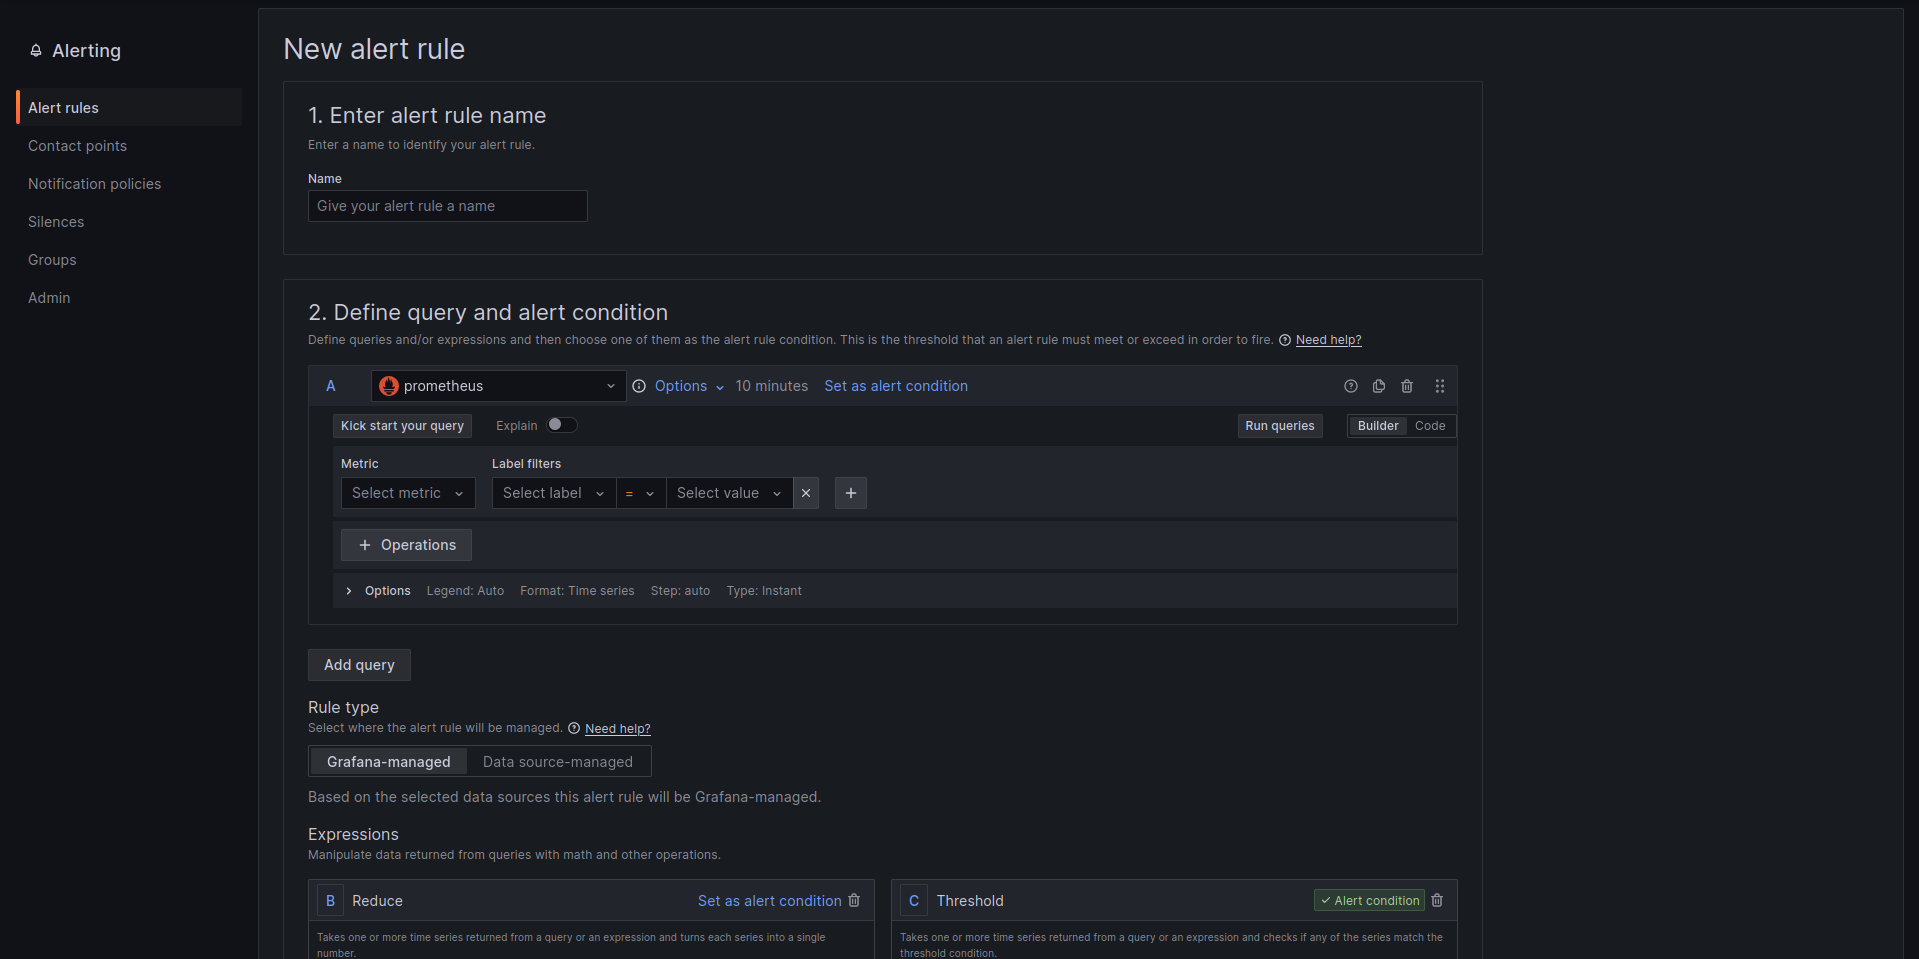
\includegraphics[width=\textwidth]{images/alerting-create}
        \caption{User Interface of creating a new alert rule in Grafana.}
        \label{fig:alerting-create}
    \end{figure}

    \section{Implemented Advanced Features}\label{sec:advanced-requirements}
    This section describes the advanced features that we implemented in our solution.
    \subsubsection{Hot/Cold Standby DBMSs}
    For MongoDB, we've implemented 2 shards with each 3 replicas. This ensures that the data is always available, even if one of the nodes fails.

    For Redis, we've implemented 1 master and 3 replicas, with the same effect as MongoDB.

    For S3, we've made use of MinIO erasure coding, ensuring data availability when one or more drives or nodes fail.

    Finally, the exact uptime requirements dictate the number of replicas the system needs. If uptime is extremely important, it may make more sense to increase the number of replicas.

    \subsubsection{Upscaling/Downscaling DBMSs}

    Using Helm Charts, we can easily scale up and down the number of replicas for each component.

    \subsubsection{Cross DBMSs Data Migration}
    For self-hosted Kubernetes solutions, data backup and migration can often be a maintainability nightmare. We would recommend taking a look at replacing the self-hosted layers to cloud managed services that provide data backups out of the box. For example, MongoDB Atlas can be used instead of the self-hosted MongoDB, which provides a fully managed MongoDB service with data backups and migration tools. Instead of MinIO, we can use AWS S3, which provides a fully managed S3 service with data backups and migration tools. For Redis, we can use AWS ElastiCache, which provides a fully managed Redis service.

    \section{Evaluation and Metrics}
    For the evaluation of this project, we've conducted several rigorous tests to ensure the system's efficacy in handling the specified requirements. We performed latency testing for the API and performed Chaos Engineering to test the fault tolerance of the system. The following sections describe the evaluation process and the results.

    \subsection{API Latency}
    For the API, we've conducted a load test using Locust, a Python framework for load testing. The test files can be found in the `load` directory. When performing the load test, we seek to see no big increase in latency. The API should automatically horizontally scale to handle the load if needed.

    The results can be seen in \Cref{fig:load-testing}. You can clearly see that around 08:03:40, the rate per second increases and the latency decreases. The same can be seen around 08:06:02. This is the Kubernetes Horizontal Pod Autoscaler (HPA) automatically scaling the number of pods in our API deployment. There were never any errors. The latency becomes relatively high before the scaler is activated, but this is not due to the limits of the HPA, but rather due to the update time of the metrics. Kubernetes by default exports metrics every 20 seconds, and the HPA takes a while to process the new metrics. The load test was conducted with 1 extra user per second, leading to a high sudden increase in request before the resource metrics are even updated. Depending on the expected user access structure (spike or gradual), this solution may suffice.

    Finally, the exact scaling requirements depend heavily on the user behaviour, environment and better defined requirements or limitations proposed by the company. The number of replicas used, or resources assigned is just set as an example.

    \begin{figure}[H]
        \centering
        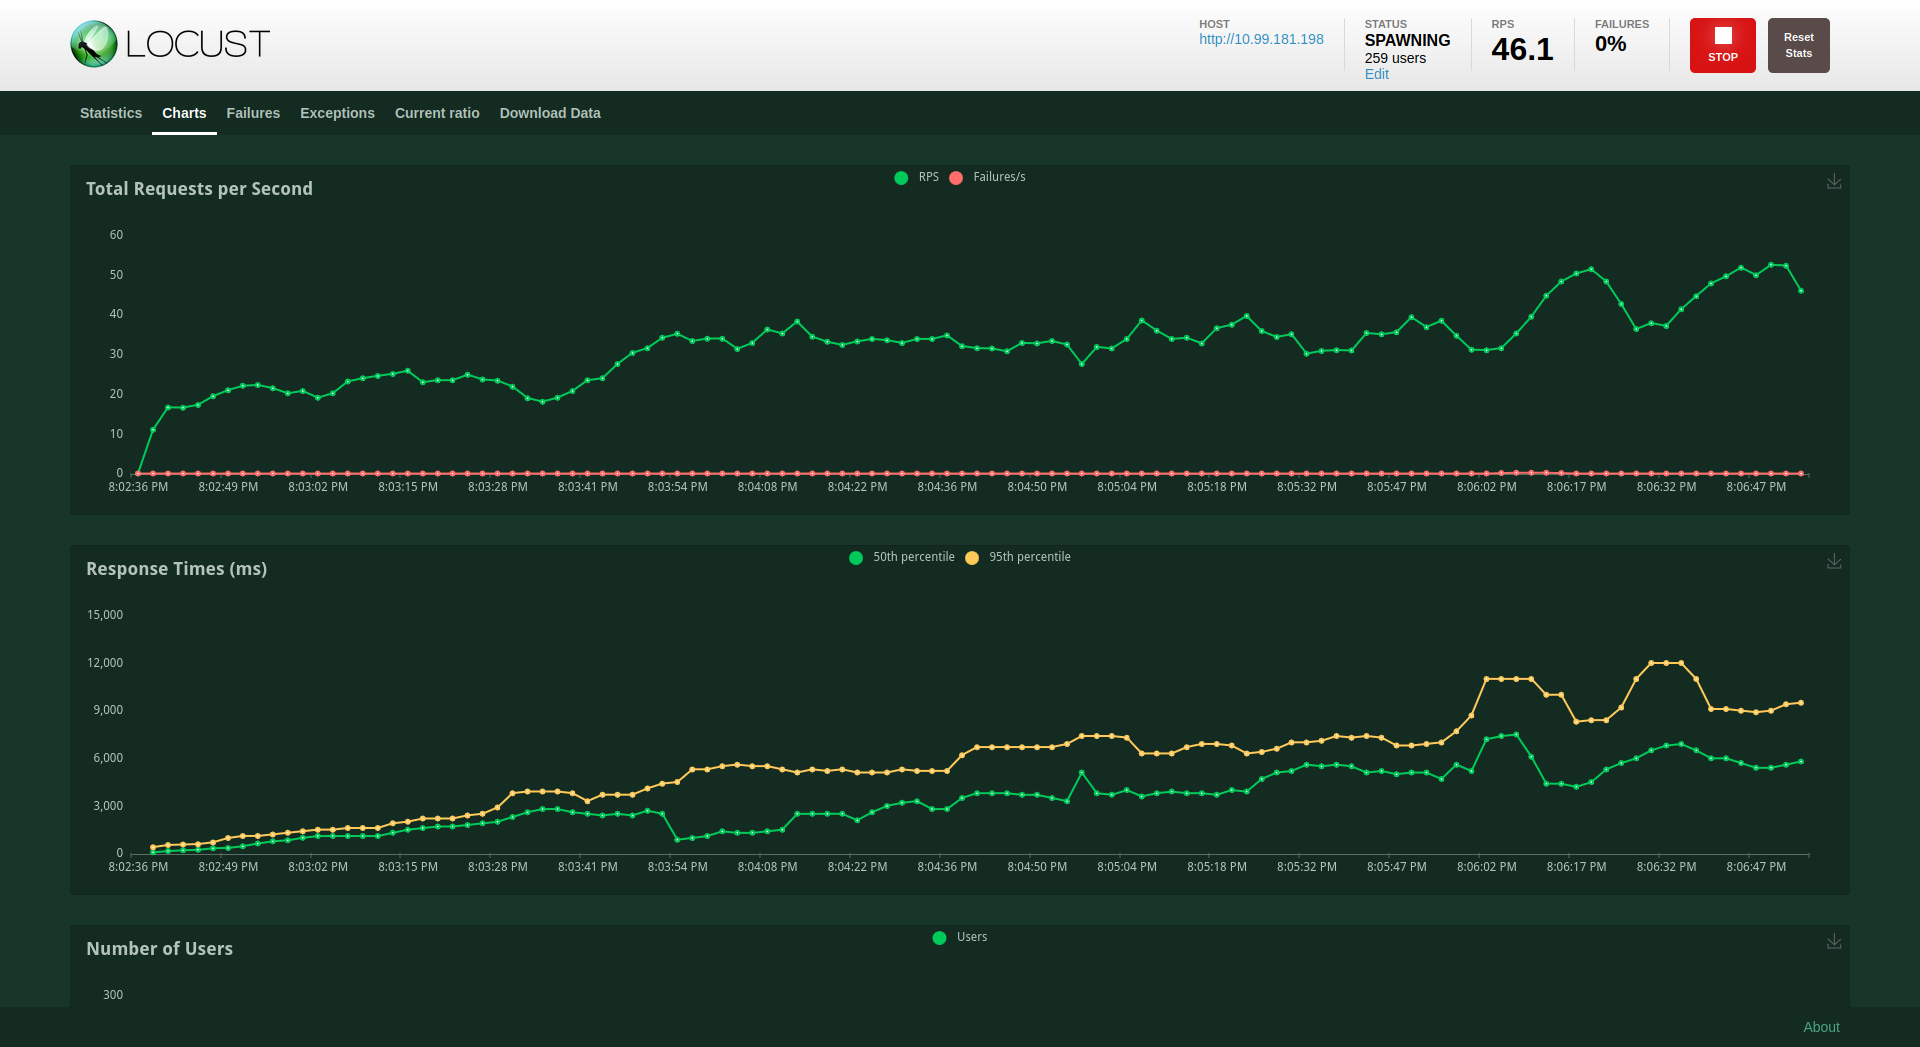
\includegraphics[width=\textwidth]{images/load-testing-success}
        \caption{API scalability testing}
        \label{fig:load-testing}
    \end{figure}

    \subsection{Disk Fault Tolerance}

    For MinIO, we've manually removed files from the drives in order to test the fault tolerance features. The `mcli admin heal` command detected the bitrot within a few minutes and restored the file. This process also runs on interval.

    \subsection{Node Fault Tolerance}

    We've tried to delete random pods in the cluster, and test the workings of the API. We sometimes see higher latency (due to the system needing to heal), but never permanent errors.

    \subsubsection{KubeDOOM}
    We've used KubeDOOM to test the fault tolerance of the system. KubeDOOM is a tool that randomly kills pods in the cluster when you play the video game DOOM. We've configured it to kill pods in each of the deployed namespaces. Just like the manual node fault tolerance test, we did not see any permanent errors.

    \begin{figure}[H]
        \centering
        
\includegraphics[width=\textwidth]{images/kubedoom}
        \caption{KubeDOOM deleting MinIO pods}
        \label{fig:kubedoom}
    \end{figure}

    \subsection{Caching}

    The integration of caching mechanisms with Redis significantly enhances the API performance. The example request in \Cref{fig:cache} shows a speedup from 26 ms to only 3 ms. The last request headers show the etag value, indicating that the response was indeed cached.

    \begin{figure}[H]
        \centering
        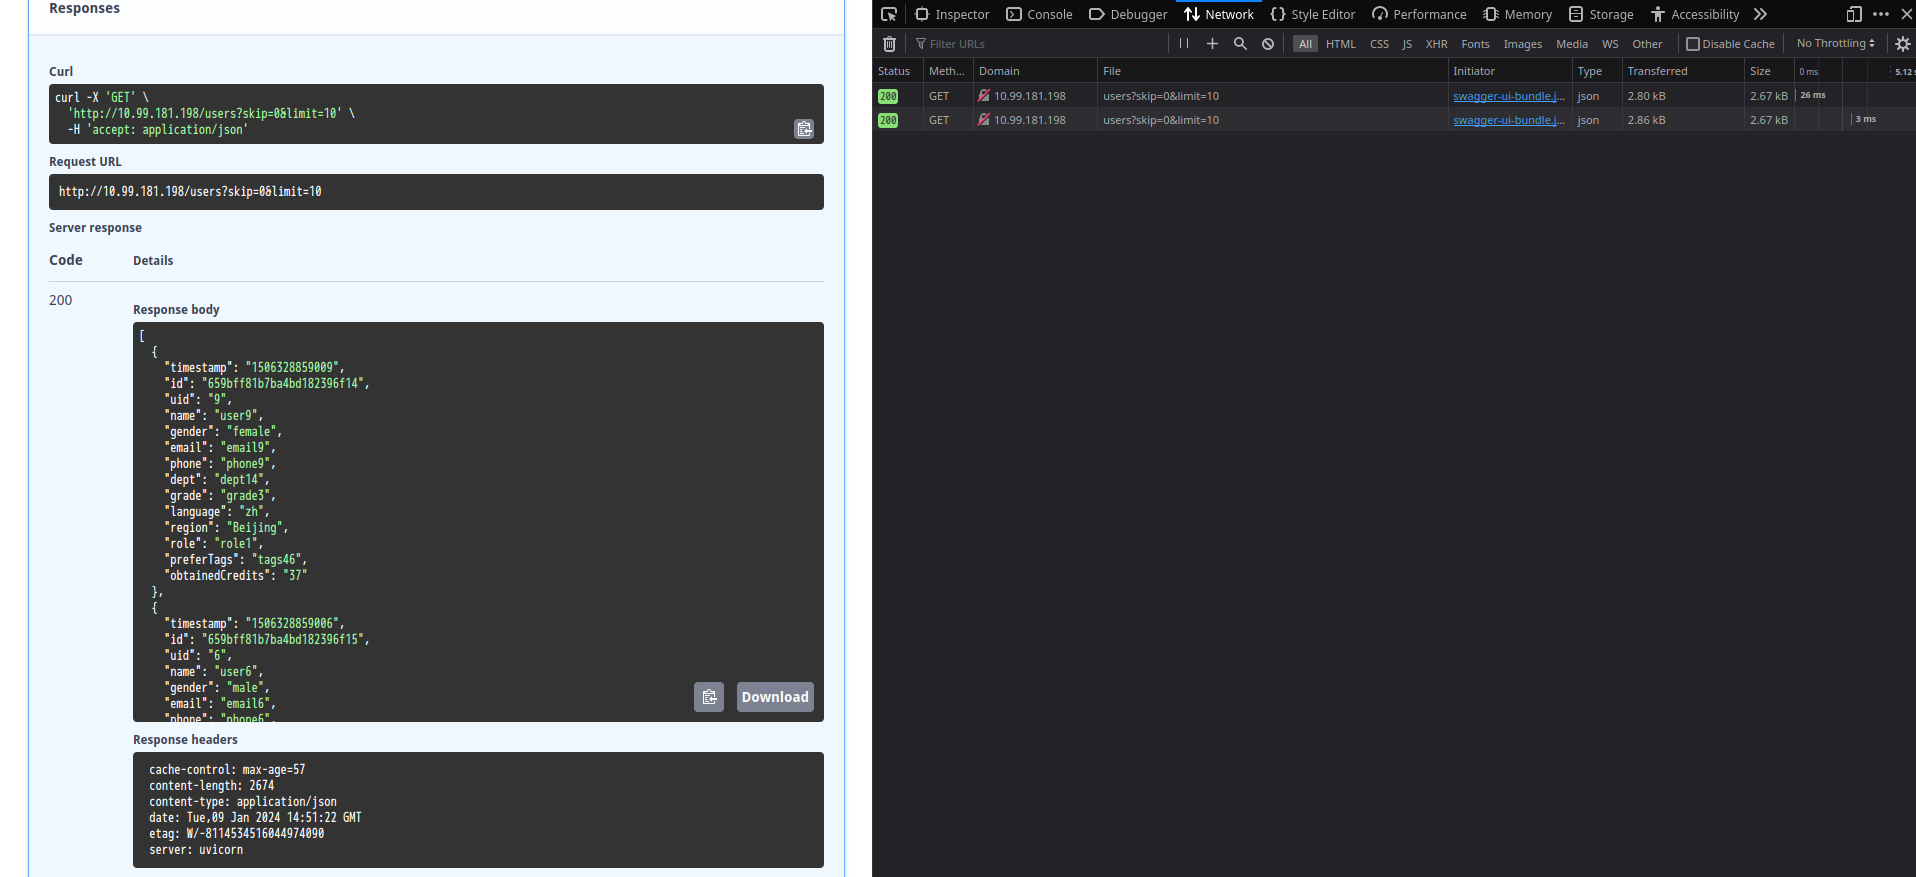
\includegraphics[width=\textwidth]{images/cache}
        \caption{Performing a request twice shows an improved latency due to caching}
        \label{fig:cache}
    \end{figure}

    In summary, the evaluation process encompasses an examination of latency, throughput, scalability, reliability, data store performance, caching efficiency, and API responsiveness. These metrics validate that the distributed database system meets the requirements of a modern scalable solution.

    \section{Conclusion}
    In conclusion, we have successfully implemented a distributed database system that meets the requirements of the project. We have also implemented several advanced features, including hot/cold standby DBMSs, upscaling/downscaling DBMSs, and cross DBMSs data migration. The system is highly performant, scalable, and reliable, with the ability to handle large volumes of data and concurrent users seamlessly. The system's efficacy in managing structured and unstructured data, and its robust caching mechanisms, ensure optimal performance and responsiveness. The integration of monitoring tools provides real-time insights into system components, enabling proactive issue identification and resolution. Overall, the system's performance tests validate its ability to meet current demands for efficient management of vast and varied data types.

    \section{Manual}
    For the manual, please see the README.md file in the root of the project. It provides instructions to get started with the deployment of our cluster. The installation instructions of each of the components and how to access them are described in their respective folders.

    Note that the manual is written for a Linux environment. For Windows, you may need to change some commands. In addition, although the manual should work out of the box, the distributed manner of the system may cause issues in some environments (e.g. different Minikube versions, VPN usage, etc.). We recommend to test the setup only if you have prior experience with Kubernetes and Docker.

    You may request us a demo environment if you are unable to get the system running.

    Versions used:
    \begin{itemize}
        \item Minikube: v1.32.0
        \item Helm: v3.13.3
        \item MongoDB: v7.0.5
        \item MongoDB Helm Chart: v7.1.6
        \item Redis: v7.2.3
        \item Redis Helm Chart: v18.5.0
        \item MinIO: v2023-09-30T07-02-29Z
        \item MinIO Helm Chart: v5.0.14
    \end{itemize}

    \section{Appendix}
    \subsection{Sharding}\label{subsec:appendix-sharding}
\begin{lstlisting}[language=python, caption=General sharding function]
const shardByKey = ({table, shardKey, shardValues}) => {
    sh.enableSharding(table);

    db[table].createIndex({[shardKey]: 1});

    shardValues.forEach(({tag, value}) => {
        sh.addTagRange(`${DB}.${table}`, {[shardKey]: value}, {[shardKey]: changeLastLetter(value)}, tag);
    });

    sh.shardCollection(`${DB}.${table}`, {[shardKey]: 1});

    db[table].getShardDistribution(); // verify chunks distributed on shards
}
\end{lstlisting}
    It can be noted that a function $changeLastLetter$ is used for the range of the shard. This is because MongoDB requires $min$ and $max$ range for each shard value, which is intuitive for numerical values, however, for string values the workaround is to change the last letter of the value to the next alphabetical letter.
\begin{lstlisting}[language=python, caption=Sharding per region and category]
const shardByRegion = (table, shardValues) => {
    shardByKey({
        table,
        shardKey: "region",
        shardValues,
    });
};

const shardByCategory = (table, shardValues) => {
    shardByKey({
        table,
        shardKey: "category",
        shardValues,
    });
};
\end{lstlisting}
\begin{lstlisting}[language=python, caption=Sharding of each collection]
shardByRegion(USERS, [
    {tag: SHARD1TAG, value: "Beijing"},
    {tag: SHARD2TAG, value: "Hong Kong"},
]);

shardByRegion(READS, [
    {tag: SHARD1TAG, value: "Beijing"},
    {tag: SHARD2TAG, value: "Hong Kong"},
]);

shardByCategory(ARTICLES, [
    {tag: SHARD1TAG, value: "science"},
    {tag: SHARD2TAG, value: "technology"},
]);

shardByCategory(ARTICLES_SCIENCE, [
    {tag: SHARD1TAG, value: "science"},
]);

shardByCategory(BE_READS, [
    {tag: SHARD1TAG, value: "science"},
    {tag: SHARD2TAG, value: "technology"},
]);

shardByCategory(BE_READS_SCIENCE, [
    {tag: SHARD2TAG, value: "technology"},
]);

shardByKey({
    table: POPULAR_RANK,
    shardKey: "temporalGranularity",
    shardValues: [
        {tag: SHARD1TAG, value: "daily"},
        {tag: SHARD2TAG, value: "weekly"},
        {tag: SHARD2TAG, value: "monthly"},
    ],
});
\end{lstlisting}
    \subsection{Aggregation Pipelines}\label{subsec:appendix-aggregation}
    Below is given the aggregation pipeline used to alternate the Read table and include region and category fields into it.
\begin{lstlisting}[language=python, caption=Aggregation pipeline for alternating Read table]
const alternateReads = () => {
    db[USERS].createIndex({id: 1});
    db[USERS].createIndex({uid: 1});
    db[ARTICLES].createIndex({aid: 1});
    db[READS].createIndex({uid: 1});
    db[READS].createIndex({aid: 1});

    db[READS].aggregate([
        {
            $lookup: {
                from: USERS,
                localField: "uid",
                foreignField: "uid",
                as: "user",
            },
        },
        {
            $lookup: {
                from: ARTICLES,
                localField: "aid",
                foreignField: "aid",
                as: "article",
            },
        },
        {
            $project: {
                _id: 1,
                timestamp: 1,
                id: 1,
                uid: 1,
                aid: 1,
                readTimeLength: 1,
                agreeOrNot: 1,
                commentOrNot: 1,
                shareOrNot: 1,
                commentDetail: 1,
                region: {
                    $getField: {
                        field: "region",
                        input: {
                            $arrayElemAt: ["$user", 0],
                        },
                    },
                },
                category: {
                    $getField: {
                        field: "category",
                        input: {
                            $arrayElemAt: ["$article", 0],
                        },
                    },
                },
            },
        },
        {
            $merge: READS,
        },
    ])
}
\end{lstlisting}
     Below is given the aggregation pipeline used to generate the Be-Read table and from the Read table.
\begin{lstlisting}[language=python, caption=Aggregation pipeline for generating Be-Read table]
const computeBeReads = () => {
    db[READS].aggregate([
    {
        $group:
            {
                _id: "$aid",
                timestamp: {$first: "$timestamp"},
                aid: {$first: "$aid"},
                category: {$first: "$category"},
                readNum: {$sum: {$toInt: "$readTimeLength"}},
                readUidList: {
                    $addToSet: {
                        $cond: {
                            if: {
                                $eq: ["$readOrNot", "1"],
                            },
                            then: "$uid",
                            else: "$REMOVE",
                        },
                    },
                },
                commentNum: {$sum: {$toInt: "$commentOrNot"}},
                commentUidList: {
                    $addToSet: {
                        $cond: {
                            if: {
                                $eq: ["$commentOrNot", "1"],
                            },
                            then: "$uid",
                            else: "$REMOVE",
                        },
                    },
                },
                agreeNum: {$sum: {$toInt: "$agreeOrNot"}},
                agreeUidList: {
                    $addToSet: {
                        $cond: {
                            if: {
                                $eq: ["$agreeOrNot", "1"],
                            },
                            then: "$uid",
                            else: "$REMOVE",
                        },
                    },
                },
                shareNum: {$sum: {$toInt: "$shareOrNot"}},
                shareUidList: {
                    $addToSet: {
                        $cond: {
                            if: {
                                $eq: ["$shareOrNot", "1"],
                            },
                            then: "$uid",
                            else: "$REMOVE",
                        },
                    },
                },
            }
    },
    {
        $out: BE_READS,
    },
],
{allowDiskUse: true})
}
\end{lstlisting}
    Below is given the aggregation pipeline used to generate the Popular-Rank table and from the Be-Read table.
\begin{lstlisting}[language=python, caption=Aggregation pipeline for generating Popular-Rank table]
const computePopularRank = () => {
    const granularity = ["day", "week", "month"];
    granularity.forEach(temporalGranularity => {
        db[BE_READS].aggregate([
            {
            $set: {
                period: {
                    $dateTrunc: {
                        date: {$toDate: {$toLong: "$timestamp"}},
                        unit: temporalGranularity
                    }
                }
            }
            },
            {
                $group: {
                    _id: "$period",
                    totalInteractions: {
                        $sum: {
                            $add: [
                                "$readNum",
                                "$commentNum",
                                "$agreeNum",
                                "$shareNum",
                            ]
                        }
                    },
                    articleAidList: {$push: "$aid"}
                }
            },
            {
                $sort: {
                    "_id": 1,
                    "totalInteractions": -1
                }
            },
            {
                $project: {
                    _id: {$toLong: "$_id"},
                    timestamp: {$toLong: "$_id"},
                    period: "$_id",
                    temporalGranularity: temporalGranularity,
                    articleAidList: 1
                }
            },
            {
                $merge: {
                    into: "popular_rank",
                }
            }
        ])
    })
}
\end{lstlisting}
\end{document}

